\section{Introduction}
Performance of join operations is crucial for relational data analytics. 
For a long time, database community has tried to improve the performance of join operations. 
The two main approaches in join algorithm designs are - partition-based and no partition-based join implementations. 

Remarkably, most of the prior work on join performance~\cite{DBLP:conf/sigmod/BlanasLP11,DBLP:conf/sigmod/SchuhCD16} has focused on a single join, usually implemented with synthetic schema and data. 
The prior work is valuable in understanding the implications of various parameters on the performance of one join operation. 
However, real life decision support queries often involve multiple join operations (multi-join), typically executed one after another on a dataset organized as star-schema or snowflake-schema. 
The debate on partitioning-based \textit{vs} no partitioning-based joins has not been extended to the settings of multi-joins. 

An additional complexity associated with analyzing multi-joins is the potential re-partitioning operation between two joins. 
The re-partitioning is needed when the input to the partitioned join is either not partitioned at all or is partitioned on a different attribute than the join attribute.

Our goal is to devise a high performance hash-based multi-join implementation algorithm for a right deep pipeline.
\reminder{Justify why we choose only hash-based implementations}.
One example of a right deep pipeline is shown in Figure~\ref{fig:right-deep-pipeline}.

\begin{figure}[t]
	\centering
	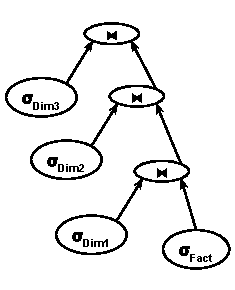
\includegraphics[]{figures/right-deep-pipeline.pdf}
		\vspace*{-1.5em}
	\caption{\textbf{A right-deep pipeline consisting of three join operations. $Dim_i$ indicates $i^{th}$ dimension table and $Fact$ denotes the fact table in a star-schema.}}
	\label{fig:right-deep-pipeline}
		\vspace*{-1.5em}
\end{figure}

An important aspect of the right-deep pipeline in Figure~\ref{fig:right-deep-pipeline} is that the build side in all the join operations is always some dimension table. 
We will leverage this aspect of the right-deep pipeline in our algorithm design. 
\reminder{Think of extending the idea to left-deep or zig-zag trees.}

Also note that Figure~\ref{fig:right-deep-pipeline} is a \textit{logical plan} produced by the optimizer. 
It gives information about join ordering. e.g. join between $Fact$ and $Dim_1$ relations should be performed first, followed by the join of the first join's result and $Dim_2$ relation. 
Figure~\ref{fig:right-deep-pipeline} does not specify the type of join (e.g. hash-based or sort-merge) and/or the partitioning nature of the join such as radix-based partitioned join or no partition-based join. 

The goal of our algorithm is to produce a high performance \textit{physical plan} which consists of the partitioning nature of each join in the pipeline.
We formally describe the problem in the next section.

\subsection{Problem Statement}
Given a right deep pipeline (as shown in Figure~\ref{fig:right-deep-pipeline}), consisting of $k$ join operations viz. $J_1, J_2, \ldots J_k$, between fact and dimension tables, find the partitioning characteristic of the implementation of each join $p(J_i)$, which can result in overall high performance of the pipeline. 

Our objective is to minimize the execution time of the multi-join pipeline. 
Let us define the execution time of join operation (probe + build phase) $J_i$ as $T(J_i)$, or simply $T_i$. 
Therefore the objective is to minimize $\sum\limits_{i=1}^{k}T_i$.

Note than if the execution exhibits pipelined parallelism, the above objective might be incorrect. 
In such a case, the total execution time for the pipeline is simply the time difference between end of execution of the last join and beginning of execution of the first join. 

We consider only two options for the partitioning characteristic of the join implementation, i.e. $p(J_i) := \textsc{partition-based}$ or $p(J_i) := \textsc{No partition-based}$. 
Thus, our problem can be viewed as an assignment problem, where we have to assign a value to $k$ binary variables.
Therefore, the size of the solution space is $2^k$, i.e. there are $2^k$ number of different possible physical plans. 

In the next section, we discuss some proposals to solve the above problem. 

\subsection{Proposed Methodology}
We first discuss the parameters involved in this problem. 
The execution time $T_i$ per join operation $J_i$ consists of both build and probe phases.
If the join implementation is partitioning-based, then the time to partition (or re-partition)the relations is included in $T_i$.

We use a metric to differentiate the performances of partitioned and non-partitioned probes. 
This metric is the number of CPU cycles per probing tuple ($C_{probe}$), and it is impacted by the size of the probed hash table $Size_{HT}$. 
In the two implementations, viz. partitioned and non-partitioned the relationship between $C_{probe}$ and $Size_{HT}$ is different. 
We study this relationship and estimate the cost of a given probe operation. 
In the next section, we present some initial empirical results to understand this relationship.

The partitioned implementation of a join operator may consist of partitioning cost. 
Therefore, we define another metric $C_{part}$, which is the number of CPU cycles spent in partitioning a single input tuple. 

Finally, we estimate the cost of each join operations in terms of CPU cycles per input tuple. 

We may use a well known technique such as dynamic programming to solve the assignment problem. 

Note that we restrict ourselves to one form of materialization of the results i.e. eager materialization. 
This means that each join operation's result is immediately materialized as soon as the operation is complete. 
(An alternative could be late materialization, as is used by MonetDB.)
\reminder{Unanswered question: Do assignment change as the query is in progress? e.g. If there are skewed results of the lower join operations in the query plan.}

\subsubsection{Heuristics}
As described earlier, the total number of possible physical plans is exponential in the number of join operations. 
It may be prohibitively expensive to analyze all possible plans. 
Therefore, we can prune the number of plans being analyzed, by applying some heuristics.
Examples of such heuristic could be: flip-flop between partitioned and non-partitioned joins is not desirable for successive join operations, prefer partitioned joins for lower level join operations in a query plan. 